\documentclass[11pt,a4paper,titlepage,french]{article}
\usepackage{ifpdf}
\usepackage[utf8]{inputenc}
\usepackage[francais]{babel}
\usepackage[T1]{fontenc}
%\usepackage[top=3cm,right=3.5cm,bottom=3cm,left=3.5cm]{geometry}
\usepackage{graphicx}

\newcommand{\HRule}{\rule{\linewidth}{0.5mm}} %Pour mettre dans la title page
\parindent 1.0cm
\setlength{\parskip}{1em plus 0.5ex minus 0.5ex}

\title{Intelligence Artificielle : Atari Go}
\author{Julien \textsc{Durillon} \and Clotilde \textsc{Massot}}
\date{\today}

%Partie pdf
\ifpdf
\pdfinfo {
	/Author (Julien Durillon - Clotilde Massot)
	/Title (Intelligence Artificielle : Atari Go)
	/Subject (Intelligence Artificielle : Atari Go)
	/Keywords (IA, go, alma)
	/CreationDate (D:20100219175732)
}
\fi
%Fin partie pdf


\begin{document}
%	\maketitle
	\begin{titlepage}

\begin{center}


% Upper part of the page

\includegraphics[scale=1.00]{./logo_fac.png}
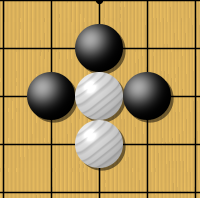
\includegraphics[scale=0.5]{./logogo.png}\\[1cm]

\textsc{\LARGE Intelligence artificielle}\\[1.5cm]

\textsc{\Large Projet TP : Atari Go}\\[0.5cm]


% Title
\HRule \\[0.4cm]
{ \huge \bfseries Étude du jeu et des possibilités d'heuristique}\\[0.4cm]

\HRule \\[1.5cm]

% Author and supervisor
\begin{minipage}{0.4\textwidth}
\begin{flushleft} \large
\emph{Auteurs :}\\[0.2cm]
\end{flushleft}
\end{minipage}

\begin{minipage}{0.5\textwidth}
\begin{flushright} \large
Clotilde \textsc{Massot}\\
Julien \textsc{Durillon}
\end{flushright}
\end{minipage}

\vfill

% Bottom of the page
{\large \today}

\end{center}
\end{titlepage}


	\tableofcontents
	\clearpage

	\abstract{Ce document explique l'étude du cas de l'atari-go dans le cadre du projet d'IA du master 1 ALMA 2010. Y sera utilisé la méthode Alpha-Beta pour gérer l'arbre des possibles.}

	\section*{Introduction}
		Le projet demandé dans ce module d'intelligence artificielle est de développer un programme capable de jouer à l'atari-go. Ce jeu est une modification du jeu de go traditionnel, jeu inventé en chine médiévale. La version d'atari-go que nous allons traiter se joue sur un goban plus petit --- d'une taille de 9x9. Le but est d'être le premier à prendre des pierres à l'adversaire. Quand une prise a été effectuée, le jeu est fini. Nous parlerons de pierres ou groupes \emph{adverses} pour désigner les pierres et groupes de l'adversaire, et \emph{alliés} pour désigner les nôtres --- i.e. ceux joués par le programme.

		Nous commencerons par expliciter notre démarche de développement, puis nous continuerons par décrire le cheminement de notre recherche sur les heuristiques, et finirons en présentant l'implémentation de l'algorithme Alpha-Beta, ainsi qu'une éventuelle interface, et les améliorations apportées et pouvant l'être.

	\section{Mise en place du projet}
		\subsection{Environnement}
		\subsection{Partage du travail}
			L'étude est faite en binôme, et les classes de description du goban ont été faites de la même façon. Le travail est ensuite partagé comme ceci : Clotilde Massot implémente dans un premier temps l'algorithme Alpha-Beta, tandis que Julien Durillon prépare la partie heuristique --- calcul de groupes de pierres\dots % Expliquer l'interface


	\section{Heuristique}

		\subsection{Un premier jet}
			Un premier indice utilisé pour déterminer l'état d'un jeu est d'identifier les groupes de pierres, et calculer leurs libertés, et noter les différents groupes en fonction de ce critère. On s'intéresse au groupe qui a le moins de libertés. Si un groupe ami a 0 liberté, le score est fixé à une valeur très basse --- $-2000$ par exemple. À l'inverse, si un groupe adverse a 0 liberté, le score est fixé à $+2000$.

			Cette méthode va entraîner une tendance à construire des longues chaînes. Il faut donc chercher une heuristique plus fine.

		\subsection{Affiner les cas gagnant ou perdant}
			Un cas gagnant --- resp. perdant --- est à première vue un cas où un groupe adverse --- resp. allié --- n'a plus aucune liberté. Mais il existe d'autres cas où un groupe est dit \emph{mort}, c'est-à-dire qu'il ne peut plus sortir vivant. Un des cas les plus évidents est le cas (c.f. figure \ref{groupemort}) où il ne reste plus qu'une libertée, et que l'adversaire est déjà autour de cette liberté.

			\begin{figure}[hbt]
			\begin{center}
			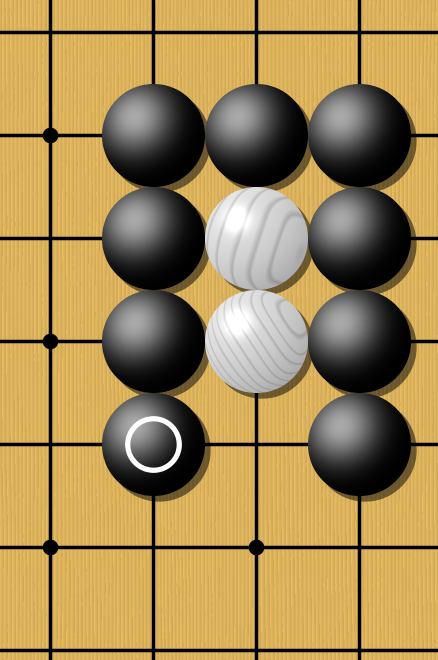
\includegraphics[width=0.4\textwidth]{groupemort.png}
			\end{center}
			\caption{Le groupe blanc est mort}
			\label{groupemort}
			\end{figure}

		\subsection{Les yeux}
			Au go, un groupe ayant deux yeux est dit imprenable --- cf. figure \ref{deuxyeux} . Un amélioration de la fonction présentée ci-dessus peut être de détecter de telles dispositions ; en effet, un groupe ayant deux yeux d'une case chacun peut n'avoir que 2 libertés tout en restant imprenable. On noterait alors mieux de tels groupes, et on aurait pas à s'en «~soucier~». Pour détecter de tels yeux, il «~suffit~» de chercher des libertés entourées uniquement du bord ou de pierres du groupe étudié. Nous pouvons assez facilement détecter des cas simples d'yeux.

			\begin{figure}[hbt]
			\begin{center}
			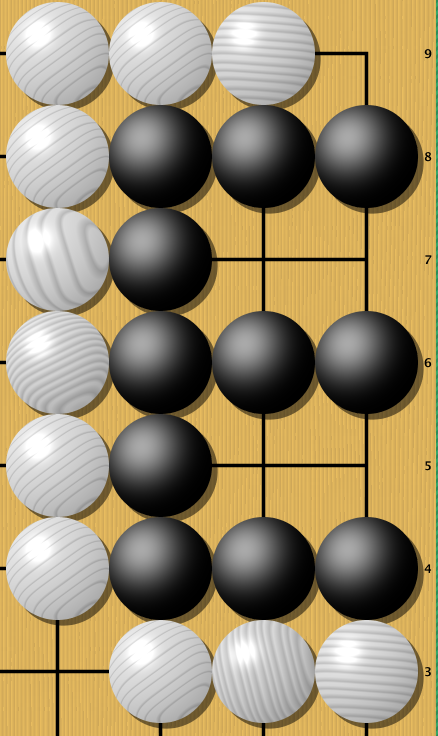
\includegraphics[width=0.4\textwidth]{deuxyeux.png}
			\end{center}
			\caption{Le groupe noir a deux yeux}
			\label{deuxyeux}
			\end{figure}

		\subsection{Les sauts}

			Une des formes intéressantes est le coup en diagonale ou \emph{kosumi} --- cf. figure \ref{kosumi}. Ce coup fait un lien entre les deux pierre qui n'existe pas encore, mais qui ne peut être coupé en un seul coup. Dans la figure \ref{kosumi}, si blanc joue dans le cercle, noir connecte dans le triangle, et vice-versa.

			\begin{figure}[hbt]
			\begin{center}
			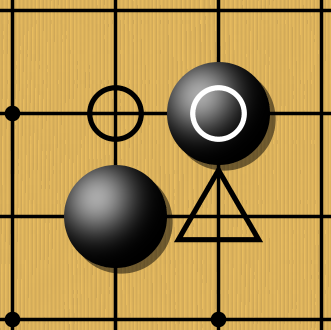
\includegraphics[width=0.3\textwidth]{kosumi.png}
			\end{center}
			\caption{Kosumi}
			\label{kosumi}
			\end{figure}

	\section{Algorithme $\alpha\beta$}
	\label{alphab}
		\subsection{Base}
			Cet algorithme se base sur l'algorithme du min-max. La base du min-max consiste à jouer un certain nombre de coup, créer un arbre représentant les possibilités de jeu, donner un score aux états de jeu atteints après génération des coups, et trouver la branche la plus intéressante. Plus un score est haut, plus le jeu est avantageux pour nous. Le parcours de l'arbre est fait en profondeur.

			Pour trouver quelle branche jouer, l'algorithme prend alternativement la branche qui a un score maximum et celle qui a un score minimum, parmi les coups possibles. Si le coup testé est joué par l'IA, la valeur maximum est choisie, car l'IA cherche à jouer le meilleur coup. Si le coup testé est joué par l'adversaire, le minimum est choisi, car l'IA considère que l'adversaire jouera le coup le pire.

		\subsection{Amélioration $\alpha\beta$}

				L'algorithme du min-max effectue l'évaluation de tous les nœuds de l'arbre de jeu d'un horizon donné. Or dans certains cas --- qui ne sont pas négligeables, l'évaluation de certains nœuds n'apporte aucun changement au processus de décision. La figure \ref{abex} va illustrer l'exemple suivant.

				\begin{figure}[hbt]
					\begin{center}
						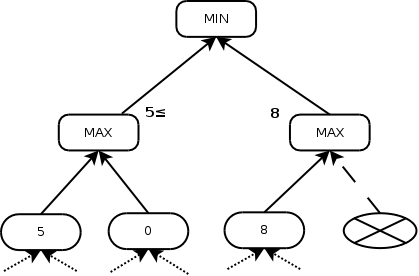
\includegraphics[width=\textwidth]{./alphabeta.png}
					\end{center}
					\caption{Exemple d'élagage $\alpha\beta$}
					\label{abex}
				\end{figure}

				L'algorithme a calculé la valeur du nœud MAX de gauche, ce nœud prend alors la valeur 5. Lorsque le deuxième nœud max est calculé, on s'apperçoit que la première valeur renvoyée --- en l'occurrence 8 --- est supérieure à 5. Or, comme l'algorithme se trouve dans un cas où il choisira la valeur maximum, le nœud MAX de gauche aura au moins la valeur 8. Donc ce n'est pas la peine d'étudier les sous-arbres suivants, car de toutes façons, c'est le 5 qui sera remonté au niveau d'au dessus.

				L'algorithme $\alpha\beta$ consiste à détecter ces cas de coupure, et donc à éviter des calculs inutiles.


		\subsection{Autres améliorations de l'algorithme}

			\subsubsection{Plusieurs fonctions d'évaluation}
				Pour améliorer cet algorithme, nous allons définir deux fonctions d'évaluation du jeu~:

				\paragraph{evaluateBeginning}
					Cette première fonction est appelée tant que moins de 6 coups ont été joués. Le grand principe de cette évaluation est de s'assurer que les coups sont joués plutôt vers le centre du goban. Comme il n'y a pas encore de groupes, ce n'est pas la peine de calculer les yeux des groupes, et moins important de compter les libertées, car il est plus difficile d'être pris au début du jeu.


				\paragraph{evaluateFollowing}
					La deuxième fonction est appelée quand le jeu a déjà bien démarré. Ici, sont testés les yeux des groupes, leurs libertés, et les sauts possibles.

			\subsubsection{Réduction des coups possibles}
				Nous considérons que certains coups n'apportent rien. Au début du jeu, on restreint les endroits où jouer à un carré excluant les deux lignes/colonnes extérieures. Pendant la suite du jeu, les possibilités  sont encores restreintes à un rectangle entourant les pierres déjà jouées agrandi de deux lignes et colonnes. Le rectangle bleu de la figure \ref{rectangletest} montre la zone qui sera testée dans le cas présenté --- les intersections situées sur les côtés du rectangle sont inclues dans la zone.

				\begin{figure}[hbt]
					\begin{center}
						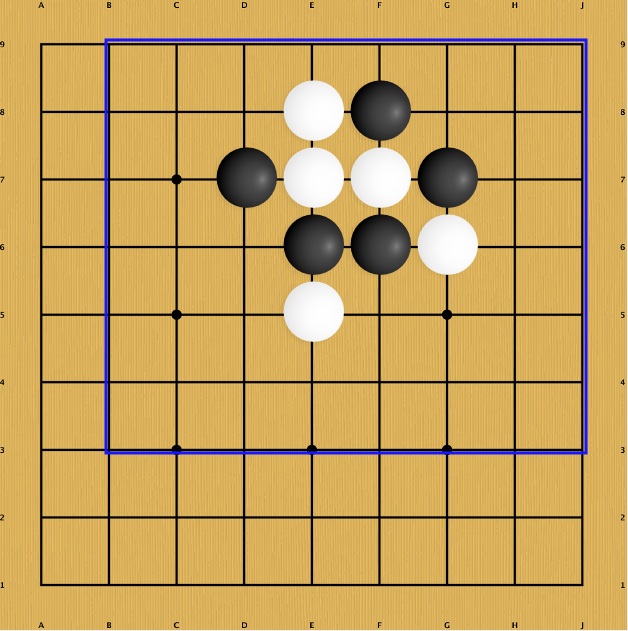
\includegraphics[width=0.7\textwidth]{./rectangle-test.png}
					\end{center}
					\caption{Zone jouable par l'ordinateur}
					\label{rectangletest}
				\end{figure}


			\subsubsection{Arrêt de l'algorithme au plus tôt}
				Nous avons ajouté une pondération de l'évaluation. Si on évalue une feuille qui est à un niveau inférieur au niveau maximum demandé, l'évaluation vaudra plus cher que si la feuille est à la profondeur maximum. Il vaut mieux jouer un très bon coup qui finit le jeu plus tôt qu'un très bon coup qui le fini plus tard.


	\section{Fonctionnement de l'application}

		\subsection{Cas d'utilisation}
			Les cas d'utilisation sont présentés dans la figure \ref{use case}.

			\begin{figure}[hbt]
				\begin{center}
					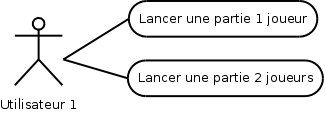
\includegraphics[width=0.7\textwidth]{./usecase.png}
				\end{center}
				\caption{Cas d'utilisation}
				\label{use case}
			\end{figure}

		Les actions possibles ne sont pas foule, car nous avons principalement orienté notre travail sur l'intelligence artificielle de l'application.

		\subsection{Diagrammes de séquence}

			\subsubsection{Partie à un joueur}
				Le déroulement d'une partie à un joueur --- contre l'ordinateur --- est décrit par la figure \ref{oneplayer}.

				\begin{figure}[hbt]
					\begin{center}
						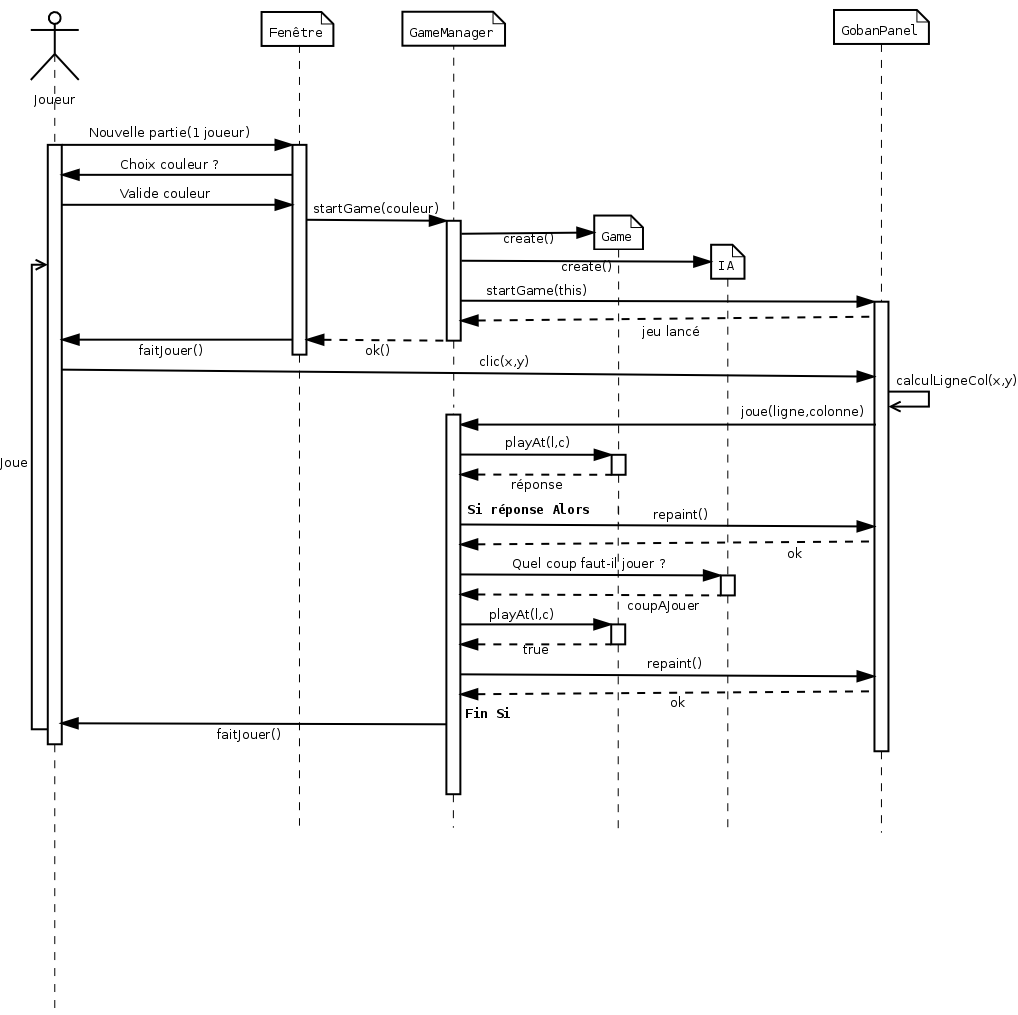
\includegraphics[width=1.2\textwidth]{./IA_1J.png}
					\end{center}
					\caption{Partie à un joueur}
					\label{oneplayer}
				\end{figure}


				Nous pouvons y distinguer des grands éléments de notre application~: La fenêtre principale, le contrôleur --- GameManager, le plateau graphique --- GobanPanel, le jeu en lui même, et la partie IA, soit l'algorithme $\alpha\beta$. L'algorithme $\alpha\beta$ a été décrit dans la section \ref{alphab}. Le jeu en lui même sera décrit dans la section \ref{howgame}.

			\subsubsection{Partie à deux joueurs}

				La figure \ref{twoplayers} décrit le déroulement d'une partie à deux joueurs.

				\begin{figure}[hbt]
					\begin{center}
						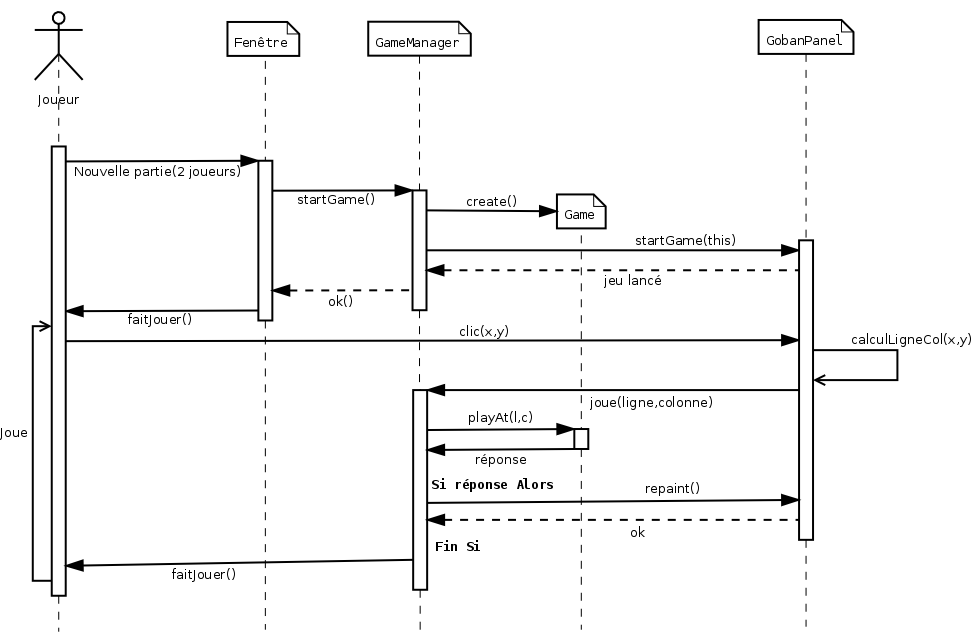
\includegraphics[width=1.2\textwidth]{./IA_2J.png}
					\end{center}
					\caption{Partie à deux joueurs}
					\label{twoplayers}
				\end{figure}


		\subsection{Le jeu : la classe Game}

			Le centre de l'application est ici la classe Game. Elle représente une partie d'atari go. Elle contient le goban courant --- état du plateau, un arbre de déroulement de la partie --- prévu pour pouvoir annuler un coup, des informations sur les groupes, leurs libertés, etc.

			Le diagramme de classes décrit par la figure \ref{classes} montre l'agencement des différents élément composant un jeu.




\end{document}
